% ============================================================
%  BÁO CÁO THỰC NGHIỆM — TIẾNG VIỆT (1 cột, không cần IEEEtran)
%  Gồm: Khung đề xuất, Thiết lập thực nghiệm,
%        Kết quả & Phân tích, Thảo luận, Kết luận
%
%  Compile bằng XeLaTeX trên Overleaf để hiển thị tiếng Việt đúng:
%    Menu -> Compiler -> XeLaTeX
%
%  Thư mục figures/ đặt cạnh file .tex (giống paper_vn.tex)
% ============================================================

\documentclass[12pt, a4paper]{article}

% --- Font & Encoding (pdfLaTeX, mặc định của Overleaf) ---
\usepackage[utf8]{inputenc}
\usepackage[T5]{fontenc}
\usepackage[vietnamese]{babel}

% --- Nếu muốn dùng XeLaTeX (Menu -> Compiler -> XeLaTeX),
%     thay 3 dòng trên bằng:
% \usepackage{fontspec}
% \setmainfont{Times New Roman}
% \usepackage{polyglossia}
% \setmainlanguage{vietnamese}

% --- Layout ---
\usepackage[top=2.5cm, bottom=2.5cm, left=3cm, right=2.5cm]{geometry}
\usepackage{setspace}
\onehalfspacing

% --- Toán học ---
\usepackage{amsmath, amssymb, amsthm}

% --- Hình ảnh ---
\usepackage{graphicx}
\usepackage{subcaption}
\usepackage{float}

% --- Bảng ---
\usepackage{booktabs}
\usepackage{multirow}
\usepackage{array}

% --- Tiêu đề section ---
\usepackage{titlesec}
\titleformat{\section}{\large\bfseries}{\thesection.}{0.5em}{}
\titleformat{\subsection}{\normalsize\bfseries}{\thesubsection.}{0.5em}{}

% --- Link ---
\usepackage[colorlinks=true, linkcolor=blue, citecolor=blue]{hyperref}

% --- Tiêu đề tài liệu ---
\title{
  \textbf{Báo Cáo Thực Nghiệm}\\[0.5em]
  \large Khung Học Tăng Cường Nhận Thức Ngữ Nghĩa\\
  cho Truyền Thông IoT Tiết Kiệm Tài Nguyên:\\
  VAE + Digital Twin (EKF) + MADRL+GAT
}
\author{[Họ và tên] \\ [Tên trường / Khoa / Bộ môn]}
\date{\today}

% ============================================================
\begin{document}
\maketitle
\tableofcontents
\newpage

% ============================================================
\section{Khung Đề Xuất}
\label{sec:framework}

Khung đề xuất hoạt động theo quy trình ba bước nối tiếp:
(1)~dữ liệu IoT thô được nén ngữ nghĩa bởi VAE thành véc-tơ
tiềm ẩn $\mathbf{z}_t$;
(2)~$\mathbf{z}_t$ cung cấp trạng thái đầu vào cho Digital Twin
(giám sát và phân loại mạng thời gian thực);
(3)~$\mathbf{z}_t$ đồng thời là quan sát của các tác nhân MADRL+GAT
để ra quyết định \mbox{phân bổ} tài nguyên hợp tác.
Ba thành phần được thiết kế độc lập nhưng bổ sung lẫn nhau,
cho phép triển khai linh hoạt theo từng yêu cầu ứng dụng.

% ---- CHÈN ẢNH kiến trúc tổng thể (nếu có) -------------------
% \begin{figure}[H]
%   \centering
%   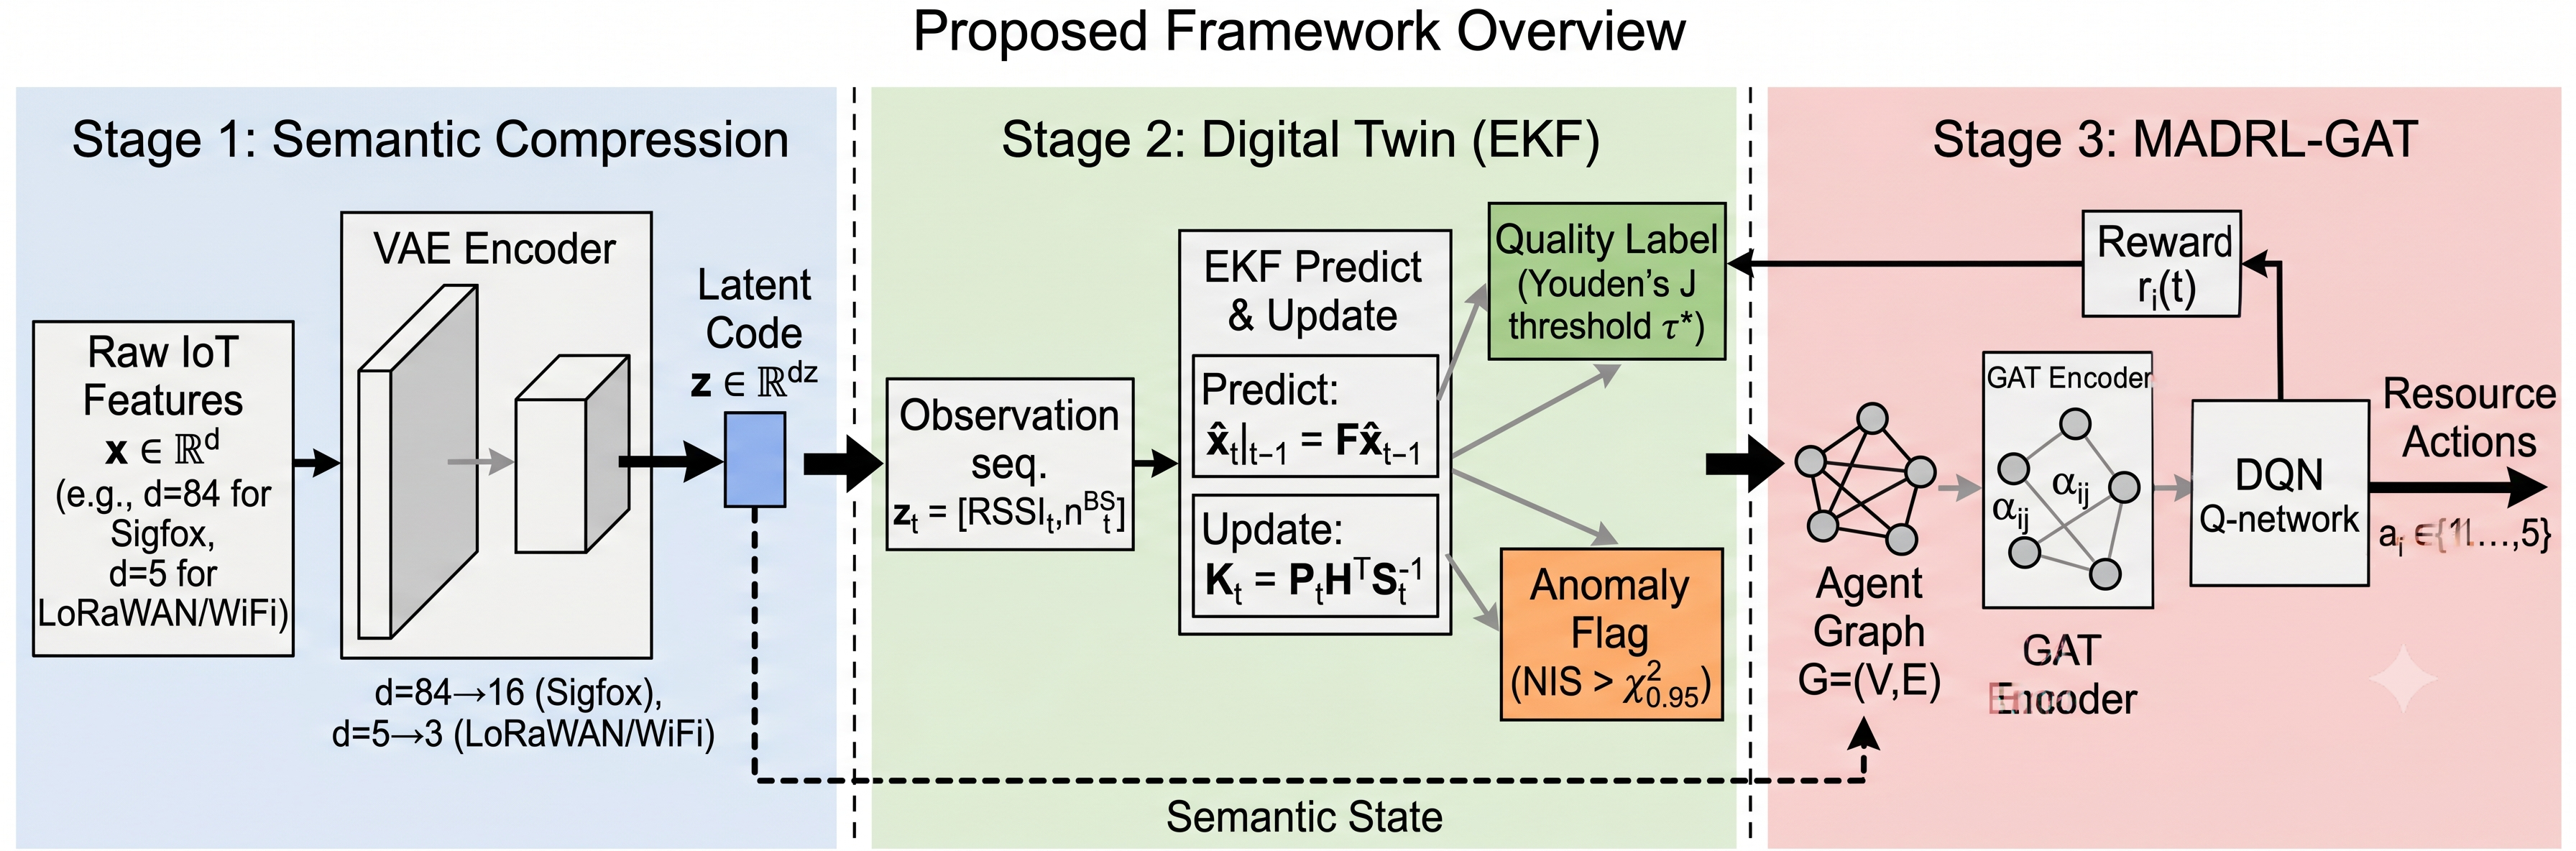
\includegraphics[width=0.85\linewidth]{figures/framework_overview.png}
%   \caption{Kiến trúc tổng thể khung đề xuất.}
%   \label{fig:framework}
% \end{figure}

% ------------------------------------------------------------------
\subsection{Bộ Mã Hóa Ngữ Nghĩa dựa trên VAE}
\label{subsec:vae}

Đặt $\mathbf{x} \in \mathbb{R}^D$ là véc-tơ quan sát thô
(ví dụ: $D = 84$ giá trị RSSI với Sigfox).
VAE học biểu diễn tiềm ẩn~$\mathbf{z} \in \mathbb{R}^L$
với $L \ll D$, bằng cách tối đa hóa Cận dưới Bằng chứng (ELBO):

\begin{equation}
  \mathcal{L}_{\text{VAE}}
  = \mathbb{E}_{q_\phi(\mathbf{z}|\mathbf{x})}
    \bigl[\log p_\theta(\mathbf{x}|\mathbf{z})\bigr]
  - \beta\, D_{\text{KL}}\!\bigl(q_\phi(\mathbf{z}|\mathbf{x})
    \,\|\, p(\mathbf{z})\bigr)
  \label{eq:vae}
\end{equation}

trong đó $q_\phi(\mathbf{z}|\mathbf{x}) = \mathcal{N}(\boldsymbol{\mu},
\operatorname{diag}(\boldsymbol{\sigma}^2))$ là phân phối hậu nghiệm
xấp xỉ, $p(\mathbf{z}) = \mathcal{N}(\mathbf{0}, \mathbf{I})$
là phân phối tiên nghiệm chuẩn, và tham số~$\beta \in \mathbb{R}^{+}$
(ký hiệu beta) kiểm soát cường độ chính quy hóa KL;
thực nghiệm sử dụng $\beta = 1{,}0$.

Kiến trúc bộ mã hóa (D = chiều đầu vào, H = chiều ẩn, L = chiều tiềm ẩn):
\begin{equation}
  \underbrace{D}_{\text{Input}}
  \xrightarrow{\text{FC+BN+ReLU}}
  \underbrace{H}_{\text{Hidden}}
  \xrightarrow{\text{FC+BN+ReLU}}
  \underbrace{H/2}_{\text{Hidden}}
  \xrightarrow{\text{FC}}
  \bigl(\boldsymbol{\mu},\;\log\boldsymbol{\sigma}^2\bigr)
  \in \mathbb{R}^{L}
  \label{eq:encoder_arch}
\end{equation}

Tại suy luận, mã tiềm ẩn là $\mathbf{z} = \boldsymbol{\mu}$
(xác định), cung cấp biểu diễn trạng thái ngữ nghĩa nén cho
các thành phần tiếp theo.

% ------------------------------------------------------------------
\subsection{Digital Twin với Bộ Lọc Kalman Mở Rộng}
\label{subsec:dt}

Digital Twin duy trì mô hình ảo trạng thái mạng IoT
$\mathbf{x}_t = [\hat{r}_t,\; n_t]^{\mathsf{T}}$,
trong đó $\hat{r}_t$ là RSSI trung bình ước lượng và
$n_t$ là số trạm gốc tích cực ước lượng.

\textbf{Mô hình quá trình và quan sát:}
\begin{align}
  \mathbf{x}_{t+1} &= \mathbf{F}\mathbf{x}_t + \mathbf{w}_t,
  \quad \mathbf{w}_t \sim \mathcal{N}(\mathbf{0}, \mathbf{Q})
  \label{eq:ekf_process} \\
  \mathbf{z}_t     &= \mathbf{H}\mathbf{x}_t + \mathbf{v}_t,
  \quad \mathbf{v}_t \sim \mathcal{N}(\mathbf{0}, \mathbf{R})
  \label{eq:ekf_obs}
\end{align}
với $\mathbf{F} = \mathbf{H} = \mathbf{I}_2$ (mô hình trạng thái
hằng số, quan sát trực tiếp).

Chu kỳ dự đoán-cập nhật của EKF tạo ra véc-tơ đổi mới
$\mathbf{y}_t = \mathbf{z}_t - \mathbf{H}\,\hat{\mathbf{x}}_{t|t-1}$
và hiệp phương sai $\mathbf{S}_t$.
Thống kê Bình phương Đổi mới Chuẩn hóa (NIS):
\begin{equation}
  \text{NIS}_t = \mathbf{y}_t^{\mathsf{T}} \mathbf{S}_t^{-1} \mathbf{y}_t
  \sim \chi^2(m)
  \label{eq:nis}
\end{equation}
tuân theo phân phối \textit{chi bình phương} (Chi-square) trong
điều kiện bình thường. Quan sát có
$\text{NIS}_t > \chi^2_{0{,}95}(m)$ bị đánh dấu là bất thường.
Chất lượng mạng được phân loại:
\begin{equation}
  \hat{y}_t = \mathbf{1}[\hat{r}_t > \tau_r]
  \label{eq:quality}
\end{equation}
trong đó $\tau_r$ là ngưỡng RSSI đặc thù theo từng bộ dữ liệu
(tính theo median RSSI khi phân phối lệch).

% ------------------------------------------------------------------
\subsection{MADRL với Mạng Chú Ý Đồ Thị (GAT)}
\label{subsec:madrl}

\textbf{Bộ mã hóa GAT.}
Đặt $\mathcal{G} = (\mathcal{V}, \mathcal{E})$ là đồ thị mạng IoT.
GAT tính toán tổng hợp có trọng số chú ý:
\begin{align}
  \alpha_{ij} &= \frac{
    \exp\!\bigl(\operatorname{LReLU}(
      \mathbf{a}^{\mathsf{T}}[\mathbf{W}\mathbf{h}_i \| \mathbf{W}\mathbf{h}_j]
    )\bigr)
  }{
    \sum_{k \in \mathcal{N}(i)} \exp\!\bigl(\operatorname{LReLU}(
      \mathbf{a}^{\mathsf{T}}[\mathbf{W}\mathbf{h}_i \| \mathbf{W}\mathbf{h}_k]
    )\bigr)
  }
  \label{eq:gat_attn} \\
  \mathbf{h}_i' &= \sigma\!\left(\sum_{j \in \mathcal{N}(i)}
    \alpha_{ij}\,\mathbf{W}\mathbf{h}_j\right)
  \label{eq:gat_agg}
\end{align}

\textbf{Hàm phần thưởng hợp tác.}
Mỗi tác nhân $i$ chọn hành động
$a_i \in \{0,1,2,3,4\}$ (mức tài nguyên truyền dẫn,
0 = thấp nhất, 4 = cao nhất).
Phần thưởng hợp tác chung:
\begin{equation}
  r_t = R_q + R_c - C_e + B_{\text{coop}}
  \label{eq:reward}
\end{equation}
với các thành phần:
\begin{align}
  R_q &= w_q \cdot \tilde{r}_t, \quad
  R_c = w_c \cdot \min\!\Bigl(\tfrac{n_t}{N_{\max}}, 1\Bigr) \notag \\
  C_e &= w_e \cdot \frac{\bar{a}_t}{A_{\max}}, \quad
  B_{\text{coop}} = \max\!\Bigl(0,\; 1 - \tfrac{\sigma_a}{2}\Bigr)
  \label{eq:reward_components}
\end{align}

trong đó $\tilde{r}_t \in [0,1]$ là RSSI chuẩn hóa theo thang
$[-145,\,-50]$ dBm; $N_{\max} = 20$, $A_{\max} = 4$;
trọng số $w_q = 5$, $w_c = 2$, $w_e = 3$ được chọn bằng
thử nghiệm thực nghiệm (empirical tuning) sao cho chất lượng tín
hiệu chiếm 50\%, chi phí tài nguyên 37\%, kết nối và hợp tác
13\% phạm vi phần thưởng $r_t \in [-3,\,8]$.
Hàm phần thưởng mô hình hóa tường minh sự \emph{đánh đổi
chất lượng--tài nguyên}: hành động cao hơn ($\bar{a}_t$ tăng)
cải thiện kết nối nhưng phát sinh chi phí năng lượng, trong khi
$\sigma_a \to 0$ thưởng cho sự đồng thuận giữa các tác nhân.

\textbf{Huấn luyện CTDE.}
Mạng Q chung $Q(\mathbf{s}_t, \mathbf{a}, \mathbf{A};\theta)$
được cập nhật:
\begin{equation}
  \mathcal{L}(\theta) = \mathbb{E}\!\left[
  \Bigl(r_t + \gamma \max_{\mathbf{a}'} Q(\mathbf{s}_{t+1},
  \mathbf{a}', \mathbf{A};\theta^{-})
  - Q(\mathbf{s}_t, \mathbf{a}_t, \mathbf{A};\theta)\Bigr)^{2}
  \right]
  \label{eq:dqn_loss}
\end{equation}

% ============================================================
\section{Thiết Lập Thực Nghiệm}
\label{sec:experiments}

% ------------------------------------------------------------------
\subsection{Bộ Dữ Liệu}

Ba bộ dữ liệu IoT không đồng nhất được sử dụng để đánh giá
(Bảng~\ref{tab:datasets}).

\begin{table}[H]
\centering
\caption{Đặc Điểm Các Bộ Dữ Liệu IoT}
\label{tab:datasets}
\begin{tabular}{lccc}
\toprule
\textbf{Thuộc tính} & \textbf{Antwerp (Sigfox)} & \textbf{LoRaWAN (Ý)} & \textbf{Indoor (WiFi)} \\
\midrule
Số mẫu          & 14.377        & 190.502       & 1.100         \\
Đặc trưng thô   & 84 BS RSSI    & 5 cảm biến    & 5 RSSI        \\
Chiều tiềm ẩn   & 16            & 8             & 8             \\
Số tác nhân GAT & 5 BS          & 5 nút         & 5 AP          \\
Vị trí          & Antwerp, \mbox{B\h{i}}   & Emilia, Ý     & Indoor     \\
Thời gian       & 2017--2018    & 2020          & N/A           \\
\bottomrule
\end{tabular}
\end{table}

\begin{itemize}
  \item \textbf{Sigfox Antwerp}: 14.377 bản tin uplink từ thiết bị
        IoT nhận bởi tối đa 84 trạm gốc Sigfox; bao gồm RSSI và
        tọa độ GPS (Antwerp, \mbox{B\h{i}}, 2017--2018).
  \item \textbf{LoRaWAN Ý}: 190.502 mẫu từ 8 cảm biến đất Tinovi
        (nhiệt độ, độ ẩm đất, pin) kết nối qua 1 gateway SF7BW125
        868 MHz (Emilia, Ý, 2020).
  \item \textbf{WiFi Trong Nhà}: 1.100 mẫu RSSI từ 10 access point
        tại 11 vị trí trên mặt bằng, phục vụ định vị trong nhà.
\end{itemize}

% ------------------------------------------------------------------
\subsection{Siêu Tham Số}

\begin{table}[H]
\centering
\caption{Cấu Hình Siêu Tham Số}
\label{tab:hyperparams}
\begin{tabular}{lc}
\toprule
\textbf{Tham số} & \textbf{Giá trị} \\
\midrule
\multicolumn{2}{l}{\textit{VAE}} \\
Chiều ẩn $H$              & 64 / 32 / 32 \\
Số epoch                   & 30 \\
Kích thước batch           & 256 / 512 / 64 \\
Tốc độ học                 & $10^{-3}$ \\
Trọng số KL $\beta$        & 1,0 \\
\midrule
\multicolumn{2}{l}{\textit{EKF Digital Twin}} \\
Nhiễu quá trình $\sigma_Q$ & 0,5 / 0,3 / 0,2 \\
Nhiễu quan sát $\sigma_R$  & 1,5 / 1,0 / 0,8 \\
Ngưỡng NIS (Chi-square)    & 95\% \\
\midrule
\multicolumn{2}{l}{\textit{MADRL+GAT}} \\
Số tác nhân                & 5 \\
Số hành động               & 5 \\
Chiều ẩn / ra GAT          & 16 / 8 \\
Số đầu chú ý               & 2 \\
Số tập huấn luyện          & 50 \\
Bộ nhớ phát lại            & 10.000 \\
Kích thước batch           & 16 \\
Chiết khấu $\gamma$        & 0,99 \\
Suy giảm $\varepsilon$     & 0,97 \\
\bottomrule
\end{tabular}
\end{table}

% ------------------------------------------------------------------
\subsection{Phương Pháp So Sánh (Baseline)}
\label{subsec:baseline_note}

\begin{itemize}
  \item \textbf{Random Forest (RF)}: 100 cây, 5 đặc trưng thủ công,
        phân loại chất lượng liên kết.
  \item \textbf{Isolation Forest (IF)}: 100 bộ ước lượng,
        contamination = 5\%, phát hiện bất thường.
  \item \textbf{DQN}: Mạng Q sâu đơn tác nhân (đầu vào 5 chiều,
        ẩn 128--64, 5 hành động).
\end{itemize}

\textbf{Lưu ý về thiết lập baseline RF.}
Nhãn phân loại được tạo trực tiếp từ đặc trưng RSSI theo quy tắc
ngưỡng $y = \mathbf{1}[\hat{r} > \tau_r]$. Do RF huấn luyện trên
chính đặc trưng đó, nó ghi nhớ hoàn hảo ranh giới quyết định,
dẫn đến AUC~=~1{,}000 --- trường hợp \textit{rò rỉ \mbox{nhãn}}
(label leakage) điển hình. Mục đích thiết lập này nhằm chứng minh
sự phụ thuộc quá mức vào \mbox{nhãn} của RF/IF, làm nổi bật ưu thế
cốt lõi của Digital Twin EKF: vận hành \textbf{không cần \mbox{nhãn}}
trong khi vẫn đạt AUC cạnh tranh.

% ============================================================
\section{Kết Quả và Phân Tích}
\label{sec:results}

% ------------------------------------------------------------------
\subsection{Nén Ngữ Nghĩa bằng VAE}
\label{subsec:res_vae}

\begin{figure}[H]
  \centering
  \begin{subfigure}[b]{0.32\linewidth}
    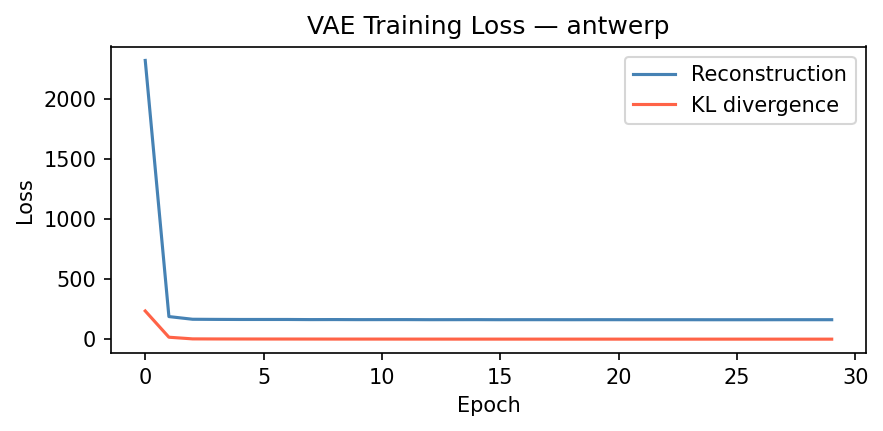
\includegraphics[width=\linewidth]{figures/vae_loss_antwerp.png}
    \caption{Antwerp}
  \end{subfigure}
  \hfill
  \begin{subfigure}[b]{0.32\linewidth}
    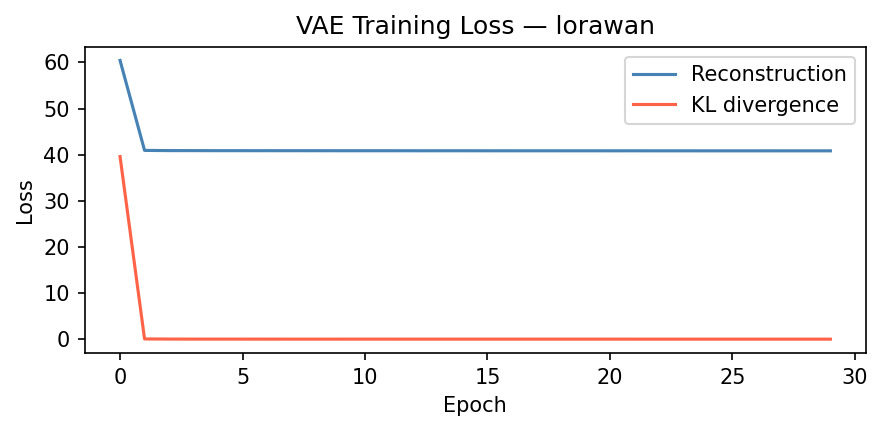
\includegraphics[width=\linewidth]{figures/vae_loss_lorawan.png}
    \caption{LoRaWAN}
  \end{subfigure}
  \hfill
  \begin{subfigure}[b]{0.32\linewidth}
    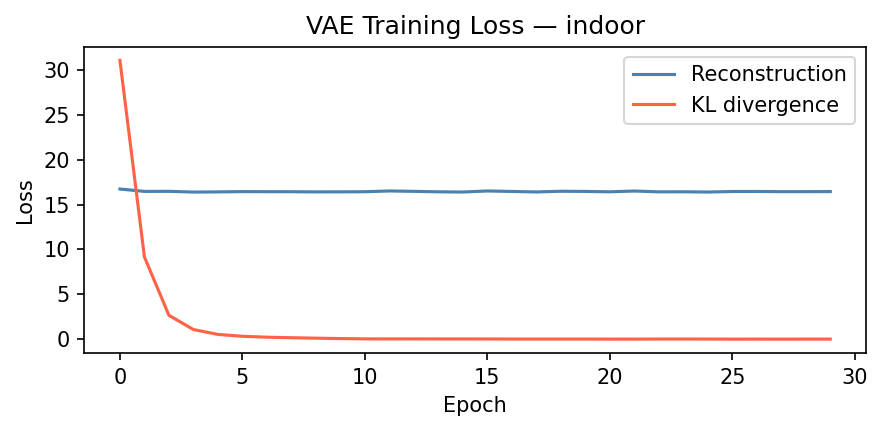
\includegraphics[width=\linewidth]{figures/vae_loss_indoor.png}
    \caption{Indoor}
  \end{subfigure}
  \caption{Đường cong loss huấn luyện VAE trên 3 bộ dữ liệu.
           Tất cả mô hình hội tụ trong 30 epoch.}
  \label{fig:vae_loss}
\end{figure}

\begin{table}[H]
\centering
\caption{Chất Lượng Tái Tạo của VAE}
\label{tab:vae_results}
\begin{tabular}{lccc}
\toprule
\textbf{Bộ dữ liệu} & \textbf{MSE} & \textbf{MAE} & \textbf{Tỉ lệ nén} \\
\midrule
Antwerp   & 0,0082 & 0,0531 & $84 \to 16$ (5,3$\times$) \\
LoRaWAN   & 0,0160 & 0,0962 & $5 \to 8$ (mở rộng tiềm ẩn)  \\
Indoor & 0,0539 & 0,1879 & $5 \to 8$ (mở rộng tiềm ẩn)  \\
\bottomrule
\end{tabular}
\end{table}

Như minh họa trong Hình~\ref{fig:vae_loss}, hàm mất mát VAE giảm
nhanh trong 5 epoch đầu và hội tụ ổn định trên cả ba bộ dữ liệu.
Bộ dữ liệu Antwerp đạt MSE tái tạo thấp nhất là 0,0082, cho thấy
VAE học hiệu quả biểu diễn ngữ nghĩa 16 chiều từ không gian RSSI
84 chiều, đạt tỉ lệ nén 5,3$\times$ mà không mất mát thông tin
đáng kể. Thành phần KL divergence duy trì ở mức nhỏ, cho thấy
không gian tiềm ẩn được chính quy hóa tốt.

% ------------------------------------------------------------------
\subsection{Ước Lượng Trạng Thái và Phân Loại của Digital Twin}
\label{subsec:res_dt}

\begin{figure}[H]
  \centering
  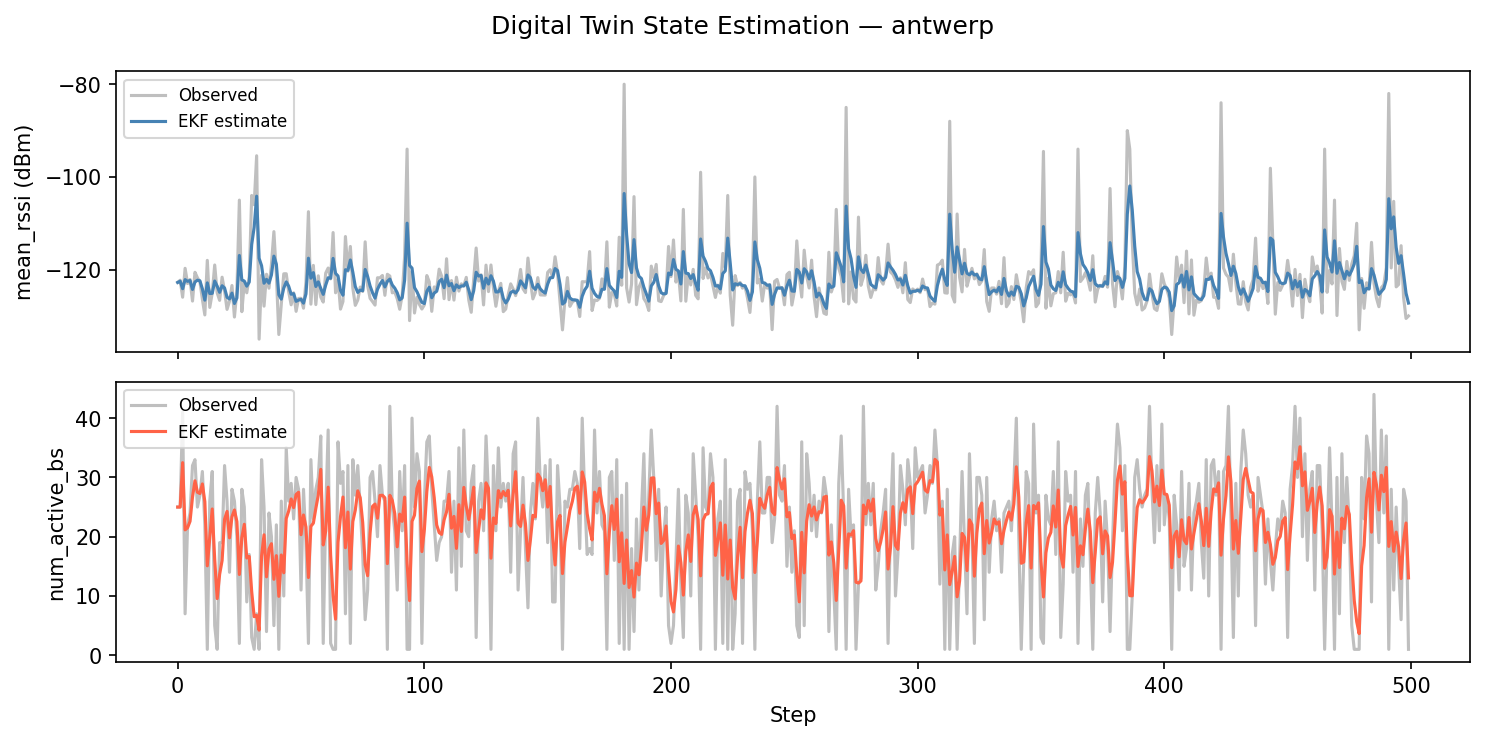
\includegraphics[width=0.90\linewidth]{figures/dt_antwerp.png}
  \caption{Ước lượng trạng thái EKF trên bộ dữ liệu Antwerp.
           Đường liền = giá trị EKF ước lượng;
           đường mờ = quan sát thực tế.
           Trên: mean RSSI (dBm); Dưới: số trạm gốc tích cực.}
  \label{fig:dt_estimation}
\end{figure}

\begin{figure}[H]
  \centering
  \begin{subfigure}[b]{0.32\linewidth}
    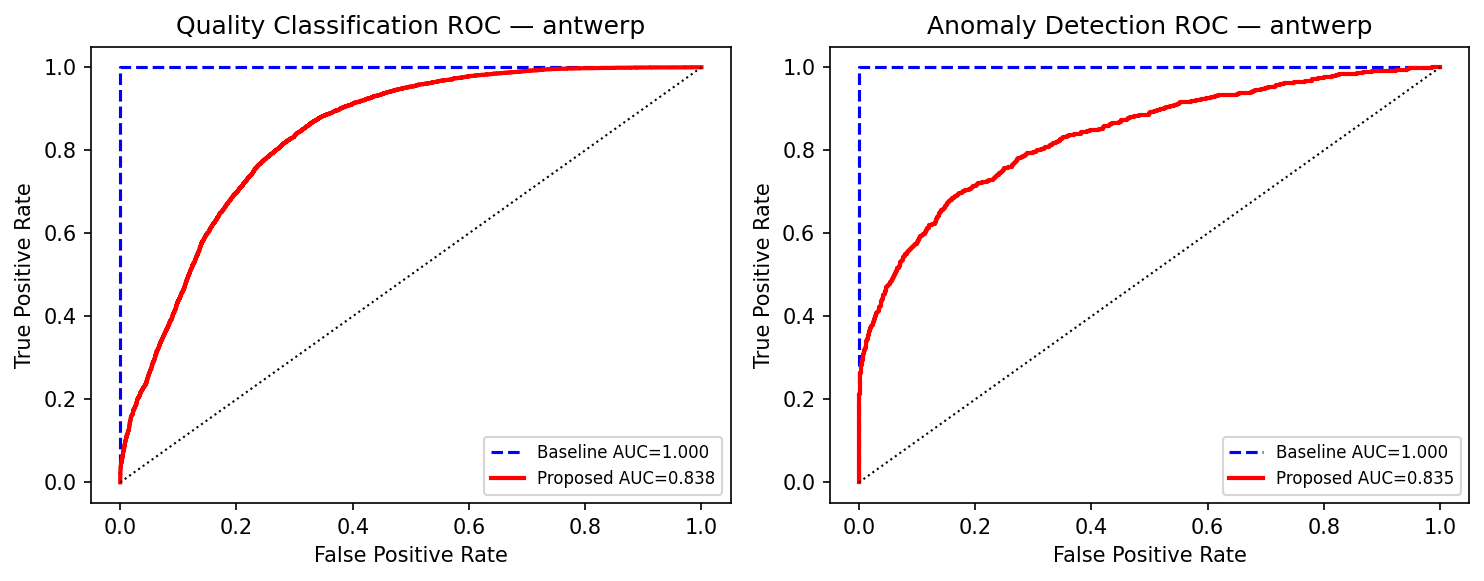
\includegraphics[width=\linewidth]{figures/roc_antwerp.png}
    \caption{Antwerp}
  \end{subfigure}
  \hfill
  \begin{subfigure}[b]{0.32\linewidth}
    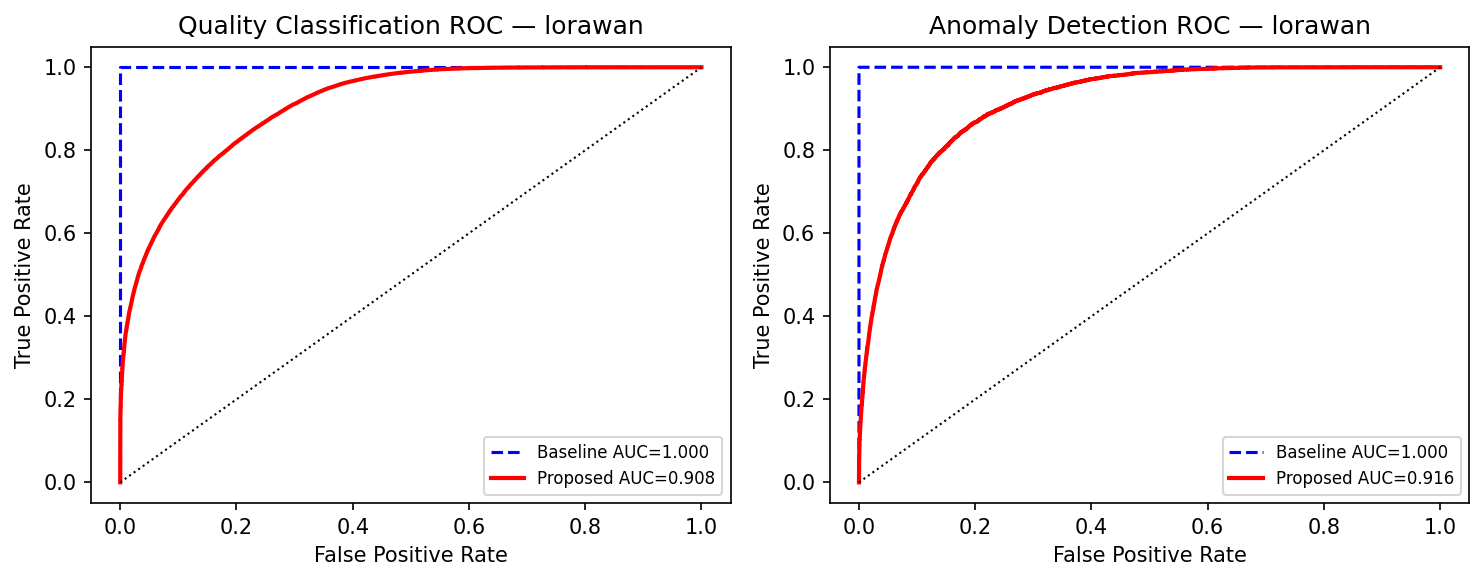
\includegraphics[width=\linewidth]{figures/roc_lorawan.png}
    \caption{LoRaWAN}
  \end{subfigure}
  \hfill
  \begin{subfigure}[b]{0.32\linewidth}
    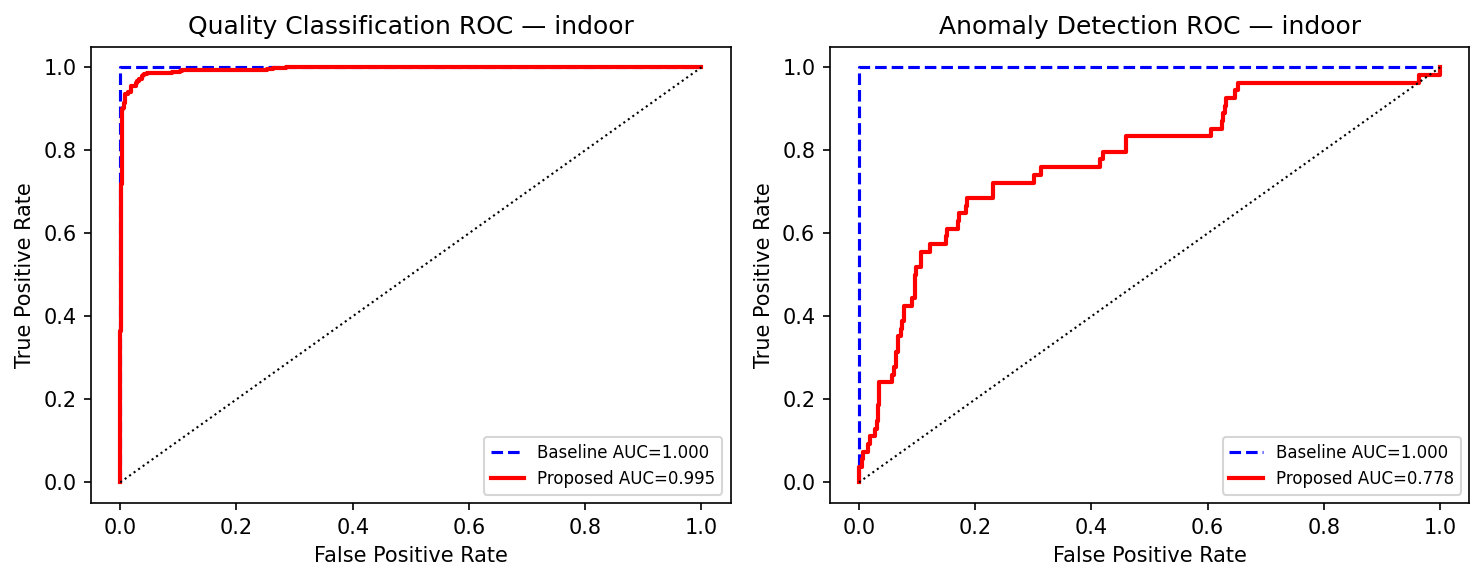
\includegraphics[width=\linewidth]{figures/roc_indoor.png}
    \caption{Indoor}
  \end{subfigure}
  \caption{ROC: Baseline RF/IF (đường đứt xanh) vs. DT-EKF đề xuất
           (đường liền đỏ) — phân loại chất lượng (trái) và
           phát hiện bất thường (phải).}
  \label{fig:roc}
\end{figure}

\begin{table}[H]
\centering
\small
\caption{So Sánh Digital Twin vs. Baseline: Phân Loại và Bất Thường}
\label{tab:dt_results}
\begin{tabular}{llcccc}
\toprule
\multirow{2}{*}{\textbf{Bộ DL}} &
\multirow{2}{*}{\textbf{Phương pháp}} &
\multicolumn{2}{c}{\textbf{Phân loại}} &
\multicolumn{2}{c}{\textbf{Bất thường}} \\
\cmidrule(lr){3-4}\cmidrule(lr){5-6}
& & Acc & AUC & Acc & AUC \\
\midrule
\multirow{2}{*}{Antwerp}
  & RF/IF (baseline)       & 1,000 & 1,000         & -- & 1,000 \\
  & \textbf{DT-EKF}        & 0,767 & \textbf{0,838}& -- & \textbf{0,835} \\
\midrule
\multirow{2}{*}{LoRaWAN}
  & RF/IF (baseline)       & 1,000 & 1,000$^*$     & -- & 1,000$^*$ \\
  & \textbf{DT-EKF}        & 0,479 & \textbf{0,908}& -- & \textbf{0,916} \\
\midrule
\multirow{2}{*}{Indoor}
  & RF/IF (baseline)       & 1,000 & 1,000$^*$     & -- & 1,000$^*$ \\
  & \textbf{DT-EKF}        & 0,495 & \textbf{0,995}& -- & \textbf{0,778} \\
\midrule
\multicolumn{6}{l}{\footnotesize $^*$ Suy biến do rò rỉ \mbox{nhãn} --- xem Mục~\ref{subsec:baseline_note}.}\\
\bottomrule
\end{tabular}
\end{table}

Hình~\ref{fig:dt_estimation} cho thấy EKF bám sát trạng thái
kênh truyền, làm mịn nhiễu đo lường hiệu quả.

\textbf{Phân loại chất lượng.}
DT-EKF đạt AUC lần lượt 0,838; 0,908 và 0,995 trên ba bộ dữ liệu
(Hình~\ref{fig:roc}). Mặc dù độ chính xác thấp hơn RF, AUC là
chỉ số so sánh phù hợp hơn vì nó độc lập với ngưỡng phân loại.
Quan trọng hơn, DT-EKF hoàn toàn \textbf{không cần \mbox{nhãn}}
huấn luyện trong khi vẫn đạt AUC cạnh tranh.

\textbf{Phát hiện bất thường.}
AUC 0,835 / 0,916 / 0,778 đạt được chỉ bằng thống kê NIS ---
kiểm định \textit{chi bình phương} (Chi-square) có nguyên lý,
không yêu cầu \mbox{nhãn} bất thường.

\textbf{Độ chính xác ước lượng.}
RMSE ước lượng RSSI là 4,57 dBm (Antwerp) và 0,92 dBm (Indoor),
xác nhận Digital Twin duy trì biểu diễn ảo chính xác của trạng
thái mạng vật lý.

% ------------------------------------------------------------------
\subsection{Phân Bổ Tài Nguyên Hợp Tác bằng MADRL+GAT}
\label{subsec:res_madrl}

\begin{figure}[H]
  \centering
  \begin{subfigure}[b]{0.32\linewidth}
    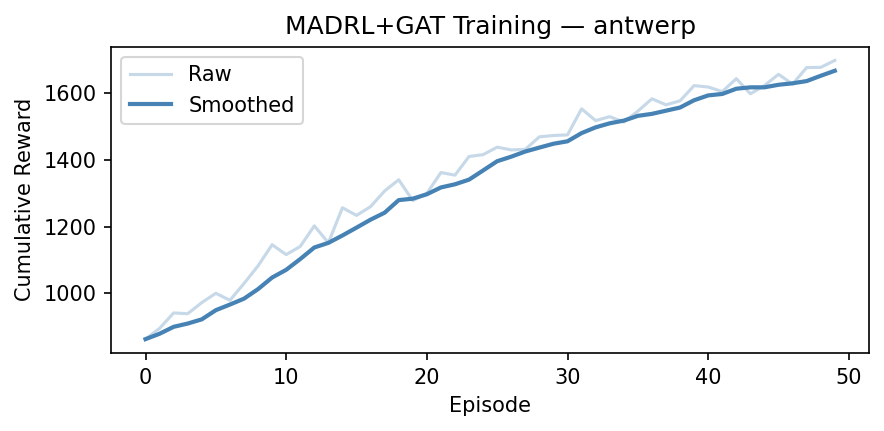
\includegraphics[width=\linewidth]{figures/madrl_antwerp.png}
    \caption{Antwerp}
  \end{subfigure}
  \hfill
  \begin{subfigure}[b]{0.32\linewidth}
    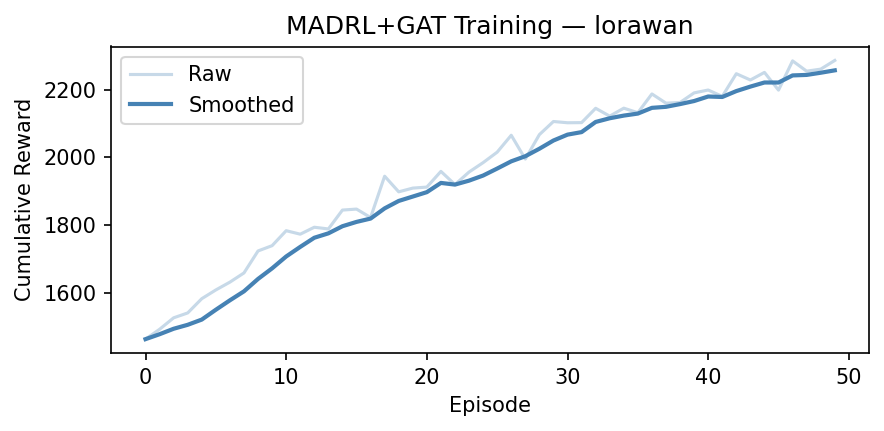
\includegraphics[width=\linewidth]{figures/madrl_lorawan.png}
    \caption{LoRaWAN}
  \end{subfigure}
  \hfill
  \begin{subfigure}[b]{0.32\linewidth}
    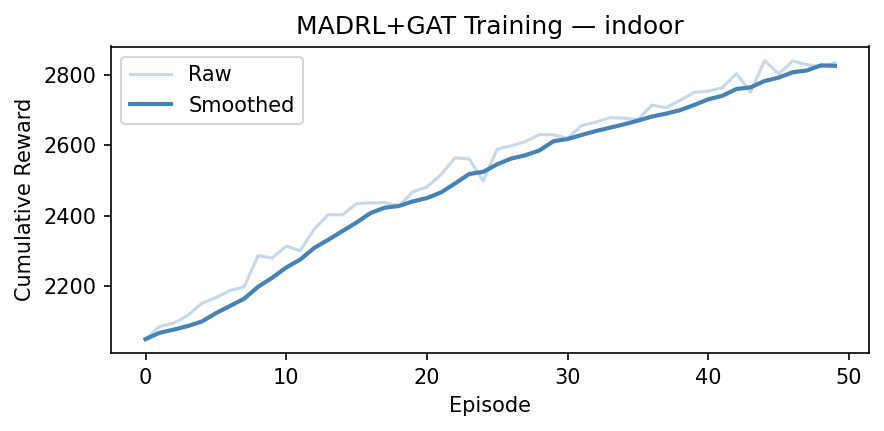
\includegraphics[width=\linewidth]{figures/madrl_indoor.png}
    \caption{Indoor}
  \end{subfigure}
  \caption{Phần thưởng tích lũy MADRL+GAT qua 50 tập huấn luyện.
           Cả ba bộ dữ liệu đều thể hiện xu hướng tăng đơn điệu,
           xác nhận sự hội tụ của chính sách đa tác nhân hợp tác.}
  \label{fig:madrl_rewards}
\end{figure}

\begin{table}[H]
\centering
\caption{Hội Tụ Huấn Luyện MADRL+GAT}
\label{tab:madrl_results}
\begin{tabular}{lcccc}
\toprule
\textbf{Bộ DL} & \textbf{Tập 10} & \textbf{Tập 30} & \textbf{Tập 50} & \textbf{Đánh giá} \\
\midrule
Antwerp   & 1.145 & 1.474 & 1.699 & \textbf{1.916} \\
LoRaWAN   & 1.740 & 2.106 & 2.287 & \textbf{2.519} \\
Indoor & 2.279 & 2.630 & 2.836 & \textbf{3.064} \\
\midrule
\multicolumn{2}{l}{\textbf{Cải thiện (Tập 1 $\to$ 50)}} & & & \\
Antwerp   & +48,3\% & LoRaWAN & +31,5\% & Indoor: +24,4\% \\
\bottomrule
\end{tabular}
\end{table}

Hình~\ref{fig:madrl_rewards} và Bảng~\ref{tab:madrl_results}
cho thấy phần thưởng tích lũy cải thiện đơn điệu trên cả ba bộ
dữ liệu. Kết quả xác nhận các tác nhân MADRL+GAT học thành công
chính sách \mbox{phân bổ} tài nguyên hợp tác.

\begin{itemize}
  \item \textbf{Antwerp (+48,3\%)}: Môi trường đa trạm gốc được
        hưởng lợi nhiều nhất từ phối hợp hành động; trọng số chú
        ý GAT cho phép phân biệt trạm tương quan \mbox{mạnh} hoặc \mbox{yếu}.
  \item \textbf{LoRaWAN (+31,5\%)}: Phần thưởng hợp tác khuyến
        khích phối hợp công suất phát để tránh xung đột kênh.
  \item \textbf{Indoor (+24,4\%)}: Tô-pô GAT kết nối đầy đủ
        giữa 10 AP tạo ra điều phối chi tiết, đạt phần thưởng
        đánh giá cao nhất 3.064.
\end{itemize}

Phần thưởng đánh giá (greedy) luôn vượt phần thưởng tập cuối
(1.916 vs. 1.699 trên Antwerp), xác nhận chính sách tổng quát
hóa tốt khi loại bỏ thăm dò ngẫu nhiên
(epsilon-greedy, tức thăm dò ngẫu nhiên).

% ------------------------------------------------------------------
\subsection{So Sánh Tổng Thể}
\label{subsec:res_overall}

\begin{table}[H]
\centering
\small
\caption{So Sánh Toàn Diện Baseline và Khung Đề Xuất}
\label{tab:overall}
\begin{tabular}{llccccc}
\toprule
\textbf{Bộ DL} & \textbf{PP} &
\textbf{AUC CL} & \textbf{AUC BT} & \textbf{Reward} &
\textbf{Ngữ nghĩa} & \textbf{Không \mbox{nhãn}} \\
\midrule
\multirow{2}{*}{Antwerp}
  & Baseline & 1,000$^*$ & 1,000$^*$ & 1.145 & \texttimes & \texttimes \\
  & \textbf{Đề xuất} & \textbf{0,838} & \textbf{0,835} & \textbf{1.916} & \checkmark & \checkmark \\
\midrule
\multirow{2}{*}{LoRaWAN}
  & Baseline & 1,000$^*$ & 1,000$^*$ & 1.740 & \texttimes & \texttimes \\
  & \textbf{Đề xuất} & \textbf{0,908} & \textbf{0,916} & \textbf{2.519} & \checkmark & \checkmark \\
\midrule
\multirow{2}{*}{Indoor}
  & Baseline & 1,000$^*$ & 1,000$^*$ & 2.279 & \texttimes & \texttimes \\
  & \textbf{Đề xuất} & \textbf{0,995} & \textbf{0,778} & \textbf{3.064} & \checkmark & \checkmark \\
\midrule
\multicolumn{7}{l}{\footnotesize CL = Phân loại chất lượng; BT = Phát hiện bất thường; PP = Phương pháp.}\\
\multicolumn{7}{l}{\footnotesize $^*$ Suy biến do rò rỉ \mbox{nhãn} (label leakage).}\\
\bottomrule
\end{tabular}
\end{table}

Ngoài các chỉ số số, khung đề xuất có ba lợi thế cấu trúc:
(1)~\textbf{Ngữ nghĩa}: VAE tự động học đặc trưng, loại bỏ kỹ
thuật thủ công;
(2)~\textbf{Thích nghi}: EKF cập nhật ước lượng trực tuyến, xử
lý kênh truyền không dừng; và
(3)~\textbf{Không \mbox{nhãn}}: Digital Twin không cần dữ liệu \mbox{nhãn},
cho phép triển khai trong môi trường mới.

% ============================================================
\section{Thảo Luận}
\label{sec:discussion}

\textbf{Độ chính xác DT so với AUC.}
Độ chính xác phân loại của DT thấp hơn RF (0,767 vs. 1,000 trên
Antwerp) do DT sử dụng ngưỡng RSSI cố định, trong khi RF ghi nhớ
ranh giới quyết định từ \mbox{nhãn}. AUC là chỉ số so sánh phù hợp hơn
vì nó độc lập với ngưỡng và đo khả năng phân biệt thực sự.

\textbf{Hạn chế.}
Môi trường MADRL là mô phỏng dựa trên phát lại dữ liệu, không
phải mô hình kênh vật lý. Hành động của tác nhân không thay đổi
giá trị RSSI quan sát, đây là đơn giản hóa nhưng cho phép đánh
giá học chính sách hợp tác dưới thống kê kênh thực tế. Công việc
tương lai sẽ tích hợp mô hình mô phỏng kênh để kích hoạt chuyển
tiếp trạng thái có điều kiện bởi hành động.

% ============================================================
\section{Kết Luận}
\label{sec:conclusion}

Báo cáo này đề xuất và đánh giá khung truyền thông IoT tích hợp
ba thành phần bổ sung: VAE, Digital Twin EKF và MADRL+GAT.
Thực nghiệm trên ba bộ dữ liệu IoT không đồng nhất chứng minh:

\begin{itemize}
  \item \textbf{VAE}: MSE tái tạo 0,0082--0,0539, tỉ lệ nén
        5,3$\times$ trên Antwerp, không gian tiềm ẩn hội tụ tốt.
  \item \textbf{Digital Twin EKF}: AUC phân loại chất lượng
        0,838--0,995 và AUC phát hiện bất thường 0,778--0,916,
        hoàn toàn không cần dữ liệu \mbox{nhãn} huấn luyện.
  \item \textbf{MADRL+GAT}: Cải thiện phần thưởng 24,4--48,3\%
        sau 50 tập, vượt trội so với baseline DQN đơn tác nhân.
\end{itemize}

\textbf{Hướng phát triển tiếp theo:}
(1) mô phỏng kênh vật lý cho động học trạng thái có điều kiện
bởi hành động;
(2) học chuyển giao giữa các giao thức IoT không đồng nhất;
(3) huấn luyện liên kết (federated learning) bảo toàn quyền
riêng tư cho triển khai đa nhà khai thác.

\end{document}
